% Created 2020-08-10 Mon 19:24
% Intended LaTeX compiler: pdflatex
\documentclass[11pt]{article}
\usepackage[utf8]{inputenc}
\usepackage[T1]{fontenc}
\usepackage{graphicx}
\usepackage{grffile}
\usepackage{longtable}
\usepackage{wrapfig}
\usepackage{rotating}
\usepackage[normalem]{ulem}
\usepackage{amsmath}
\usepackage{textcomp}
\usepackage{amssymb}
\usepackage{capt-of}
\usepackage{hyperref}
\author{Nick}
\date{\today}
\title{Hamilton Temp Analysis}
\hypersetup{
 pdfauthor={Nick},
 pdftitle={Hamilton Temp Analysis},
 pdfkeywords={},
 pdfsubject={},
 pdfcreator={Emacs 26.3 (Org mode 9.4)}, 
 pdflang={English}}
\begin{document}

\maketitle
\tableofcontents


\section{Summer trend in minimum temperature starting in 1990}
\label{sec:orgcf966ed}

It is true that if we look at the Hamilton weather station data from 1990 to
present that there is a decreasing trend in minimum temperature over that time
period. This is the time period that Bruce originally used for his evaluation.

\begin{center}
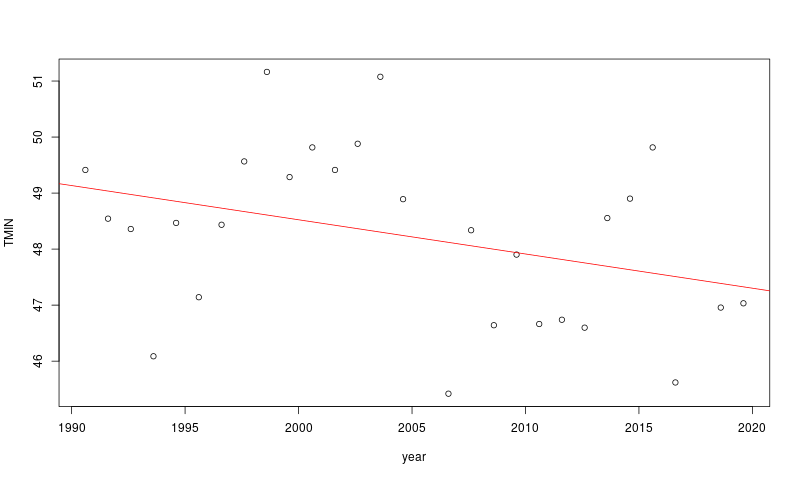
\includegraphics[width=.9\linewidth]{summer_tmin_1990.png}
\end{center}

And the trend is fairly significant (p = 0.07). The summary statistics on that
trend look like this:

\begin{verbatim}
summary(mod1)
\end{verbatim}

\begin{verbatim}

Call:
lm(formula = paste(var.nm, " ~ year"), data = metv.season)

Residuals:
    Min      1Q  Median      3Q     Max 
-2.8268 -1.0954 -0.1639  0.9188  2.7730 

Coefficients:
              Estimate Std. Error t value Pr(>|t|)    
(Intercept)  5.036e+01  1.159e+00  43.458   <2e-16 ***
year        -1.672e-04  8.886e-05  -1.882   0.0711 .  
---
Signif. codes:  0 ‘***’ 0.001 ‘**’ 0.01 ‘*’ 0.05 ‘.’ 0.1 ‘ ’ 1

Residual standard error: 1.482 on 26 degrees of freedom
Multiple R-squared:  0.1199,	Adjusted R-squared:  0.086 
F-statistic: 3.541 on 1 and 26 DF,  p-value: 0.07112
\end{verbatim}

\section{Summer trend in minimum temperature starting in 1980}
\label{sec:orgb6fe431}

However, if we just add 10-years to the data by going back to 1980, take a look
at what happens to the trend.

\begin{center}
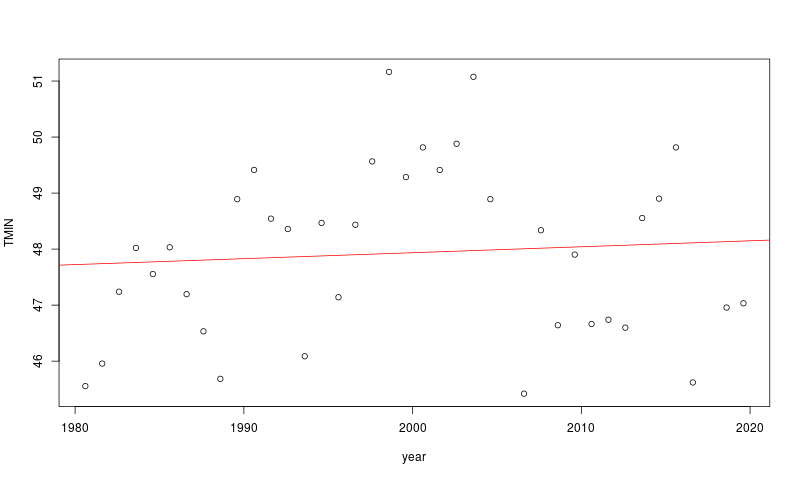
\includegraphics[width=.9\linewidth]{summer_tmin_1980.png}
\end{center}

In this case the trend is not significant, but is actually increasing:

\begin{verbatim}
summary(mod2)
\end{verbatim}

\begin{verbatim}

Call:
lm(formula = paste(var.nm, " ~ year"), data = metv.season)

Residuals:
    Min      1Q  Median      3Q     Max 
-2.5871 -1.3083  0.2544  1.0256  3.2416 

Coefficients:
             Estimate Std. Error t value Pr(>|t|)    
(Intercept) 4.762e+01  6.916e-01  68.847   <2e-16 ***
year        2.908e-05  5.984e-05   0.486     0.63    
---
Signif. codes:  0 ‘***’ 0.001 ‘**’ 0.01 ‘*’ 0.05 ‘.’ 0.1 ‘ ’ 1

Residual standard error: 1.542 on 36 degrees of freedom
Multiple R-squared:  0.006515,	Adjusted R-squared:  -0.02108 
F-statistic: 0.2361 on 1 and 36 DF,  p-value: 0.63
\end{verbatim}

\section{Summer trend in minimum temperature starting in 1950}
\label{sec:orgbb9106f}

The standard time period for evaluating historical trends starts in 1950. If we
use this as our starting point the trend looks very similar to the trend
starting in 1980. Slightly increasing but statistically insignifcant.

\begin{center}
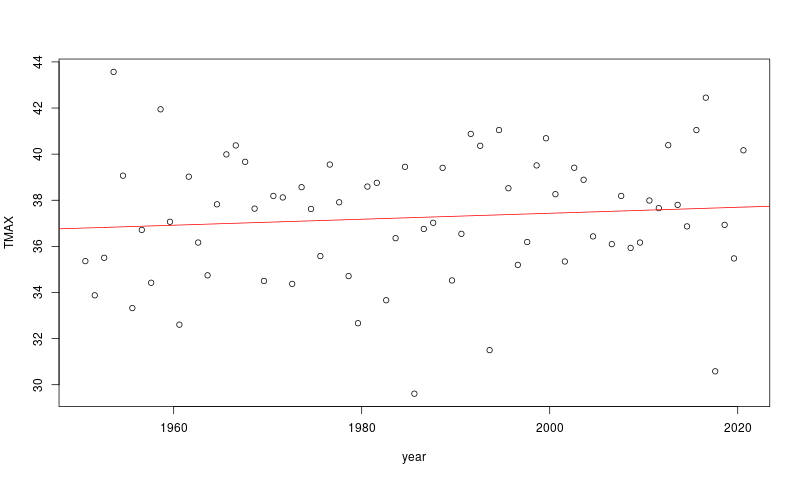
\includegraphics[width=.9\linewidth]{summer_tmin_1950.png}
\end{center}

\begin{verbatim}
summary(mod3)
\end{verbatim}

\begin{verbatim}

Call:
lm(formula = paste(var.nm, " ~ year"), data = metv.season)

Residuals:
     Min       1Q   Median       3Q      Max 
-2.59886 -0.93249 -0.04234  0.90798  3.15724 

Coefficients:
             Estimate Std. Error t value Pr(>|t|)    
(Intercept) 4.796e+01  2.036e-01 235.536   <2e-16 ***
year        4.247e-06  2.270e-05   0.187    0.852    
---
Signif. codes:  0 ‘***’ 0.001 ‘**’ 0.01 ‘*’ 0.05 ‘.’ 0.1 ‘ ’ 1

Residual standard error: 1.364 on 66 degrees of freedom
Multiple R-squared:  0.0005301,	Adjusted R-squared:  -0.01461 
F-statistic: 0.035 on 1 and 66 DF,  p-value: 0.8522
\end{verbatim}

All other trends (seasons and variables) are increasing at the Hamilton station
when you evaluate them from 1950. See below for figures and statistics.

\section{Summer trend in maximum temperature starting in 1950}
\label{sec:org0427e6f}
\begin{center}
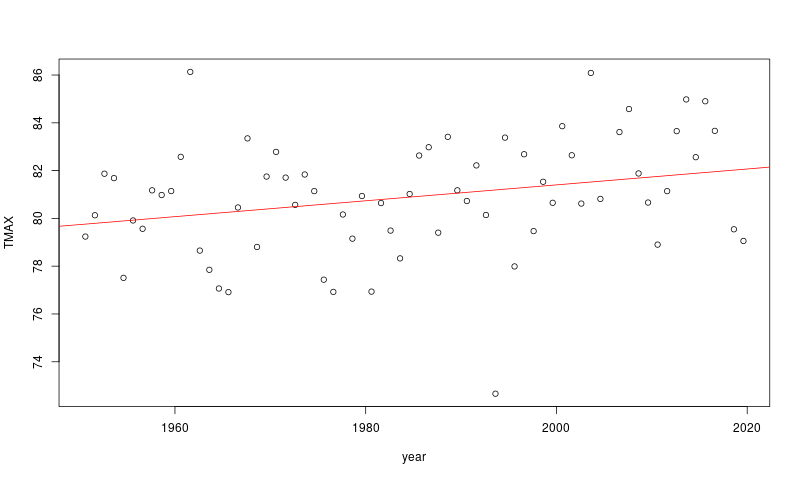
\includegraphics[width=.9\linewidth]{summer_tmax_1950.png}
\end{center}


\begin{verbatim}
summary(mod4)
\end{verbatim}

\begin{verbatim}

Call:
lm(formula = paste(var.nm, " ~ year"), data = metv.season)

Residuals:
    Min      1Q  Median      3Q     Max 
-8.5280 -1.5163  0.1465  1.7059  6.0032 

Coefficients:
             Estimate Std. Error t value Pr(>|t|)    
(Intercept) 8.041e+01  3.506e-01 229.351   <2e-16 ***
year        9.101e-05  3.908e-05   2.329   0.0229 *  
---
Signif. codes:  0 ‘***’ 0.001 ‘**’ 0.01 ‘*’ 0.05 ‘.’ 0.1 ‘ ’ 1

Residual standard error: 2.348 on 66 degrees of freedom
Multiple R-squared:  0.07593,	Adjusted R-squared:  0.06193 
F-statistic: 5.423 on 1 and 66 DF,  p-value: 0.02294
\end{verbatim}

\section{Winter trend in minimum temperature starting in 1950}
\label{sec:org9cc9ccd}

\begin{center}
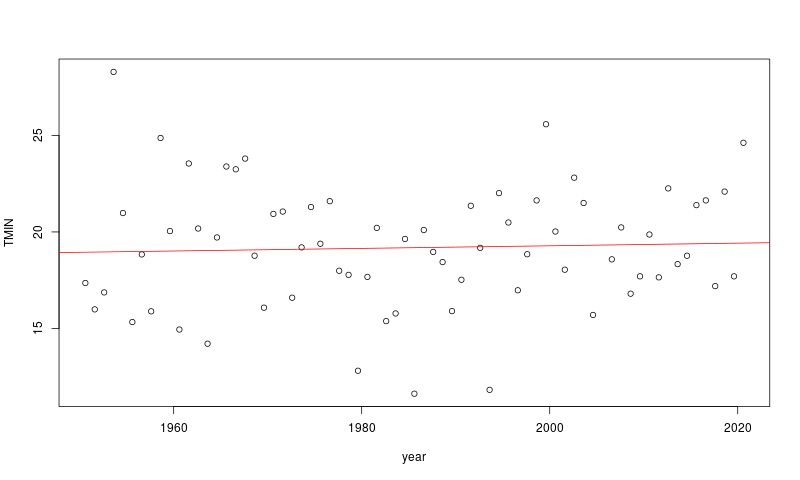
\includegraphics[width=.9\linewidth]{winter_tmin_1950.png}
\end{center}

\begin{verbatim}
summary(mod5)
\end{verbatim}

\begin{verbatim}

Call:
lm(formula = paste(var.nm, " ~ year"), data = metv.season)

Residuals:
    Min      1Q  Median      3Q     Max 
-7.5648 -2.0013 -0.1073  2.0961  9.3177 

Coefficients:
             Estimate Std. Error t value Pr(>|t|)    
(Intercept) 1.908e+01  4.756e-01  40.124   <2e-16 ***
year        1.846e-05  5.088e-05   0.363    0.718    
---
Signif. codes:  0 ‘***’ 0.001 ‘**’ 0.01 ‘*’ 0.05 ‘.’ 0.1 ‘ ’ 1

Residual standard error: 3.187 on 68 degrees of freedom
Multiple R-squared:  0.001932,	Adjusted R-squared:  -0.01275 
F-statistic: 0.1316 on 1 and 68 DF,  p-value: 0.7179
\end{verbatim}

\section{Winter trend in maximum temperature starting in 1950}
\label{sec:org09c73f0}

\begin{center}
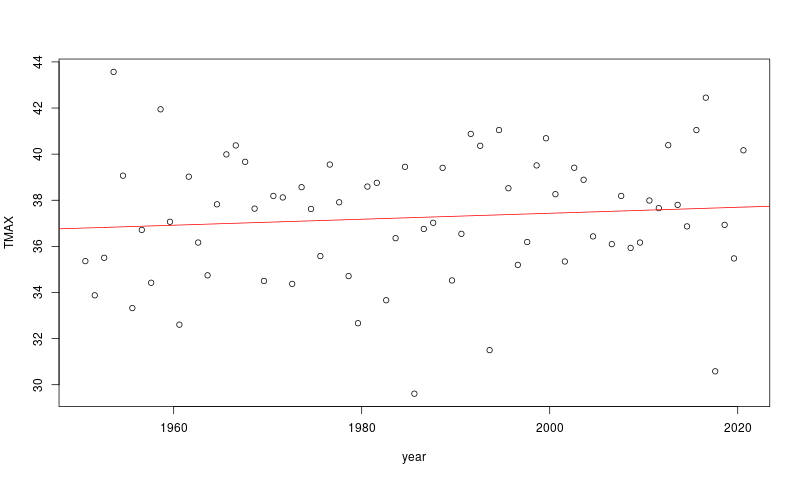
\includegraphics[width=.9\linewidth]{summer_tmin_1950.png}
\end{center}


\begin{verbatim}
summary(mod6)
\end{verbatim}

\begin{verbatim}

Call:
lm(formula = paste(var.nm, " ~ year"), data = metv.season)

Residuals:
    Min      1Q  Median      3Q     Max 
-7.6401 -1.5973  0.1692  2.0891  6.7300 

Coefficients:
             Estimate Std. Error t value Pr(>|t|)    
(Intercept) 3.705e+01  4.156e-01  89.136   <2e-16 ***
year        3.547e-05  4.447e-05   0.798    0.428    
---
Signif. codes:  0 ‘***’ 0.001 ‘**’ 0.01 ‘*’ 0.05 ‘.’ 0.1 ‘ ’ 1

Residual standard error: 2.786 on 68 degrees of freedom
Multiple R-squared:  0.009269,	Adjusted R-squared:  -0.0053 
F-statistic: 0.6362 on 1 and 68 DF,  p-value: 0.4279
\end{verbatim}
\end{document}
